\documentclass[book,10pt,twoside,twocolumn,openany]{dndbook}
\usepackage[german]{babel}

\usepackage[utf8]{inputenc}
\usepackage{hang}
\usepackage{lipsum}
\usepackage{listings}

\usepackage{blindtext}
%\usepackage[explicit]{titlesec}
\usepackage{todonotes}

% change part format
\titleformat{\part}[drop]{}{}{0pt}{}
\titlespacing*{\part}{0pt}{0pt}{0pt}


\newcommand\hide[1]{%
  \refstepcounter{section}%
  \addcontentsline{toc}{section}{\protect\numberline{\thesection}#1}%
  \sectionmark{#1}
}

\lstset{%
  basicstyle=\ttfamily,
  language=[LaTeX]{TeX},
}
\cfoot{\_ \\ dnd-gg.github.io}
\chead{}
\title{
 \centering
\includegraphics[width=12cm]{img/logo}\\Dungeons And Dragons\\\small Grundregeln und Notizen\\\small ein schneller DnD Einstieg für neue Spieler}
\date{\today}

% Start document
\begin{document}

\maketitle
\tableofcontents
\chapter{Kapitel 1: Charakter}
\section{Charakter-Erstellung}
\subsection{Volk wählen}
Wähle ein Volk und schreibe die folgenden Werte, Volksmerkmale und Informationen (teilweise auch aus aus den Beschreibungen im PH) auf:
\begin{itemize}
  \item erhöhung der Attributwerte
  \item Alter
  \item Gesinnung
  \item Größe
  \item Bewegungsrate
  \item Sprachen
\end{itemize}

\subsection{Klasse wählen}
Wähle eine Klasse und schreibe die folgenden Werte und Informationen aus den Beschreibungen im PH auf:
\begin{itemize}
  \item Vorzüge/Klassenmerkmale
  \item Übungsbonus
  \item Trefferwürfel
    \subitem \textit{(Völkerbonus:siehe Tabelle PH S.12)}
\end{itemize}

\subsection{Stufen}
Einigt euch auf eine Stufe eurer Charaktere. \\
\textit{Empfohlen: Stufe 1, 0 EP}\\
\textit{für die Stufentabelle: PH S. 15}

\subsection{Attributwerte}
Es Existieren folgende Attributwerte die bestimmt werden müssen.
\begin{itemize}
  \item Stärke
  \item Geschwindigkeit
  \item Konstitution
  \item Intelligenz
  \item Weisheit
  \item Charisma
\end{itemize}
Dafür gibt es zwei Varianten:

\subsubsection{Generierung}
\subsubsection{\small Schritt 1}
Wiederhole diesen Vorgang 6 Mal:
\begin{itemize}
  \item Würfel vier mal w6
  \item nehme die höchsten drei Werte
  \item addiere sie
  \item schreibe sie auf
\end{itemize}
Du kannst auch alternativ die Werte \\ \textit{15, 14, 13, 12, 10, 8} \\ verwenden, wenn du Zeit sparen möchtest.
\subsubsection{\small Schritt 2}
Weise nun jeden Wert einem Attribut zu.

\subsubsection{\small Schritt 3}
Wende die Volksmodifizierung an die im PH bei jedem Volk beschrieben steht.

\subsubsection{\small Schritt 4}
Berechne die Attributmodifikatoren. Diese Berechnest du wie folgt:

$$\frac{Attributwert-20}{2}$$

\subsubsection{Attribute Masschneidern}
\textit{Nur wenn der DM einverstanden ist.}\\
Beim Attribute Masschneidern hat jeder Spieler 27 Kosten-Punkte zur Verfügung und darf sich die Werte selber zuweisen.
  \begin{dndtable}[cc]
  \textbf{Werte} & \textbf{Kosten} \\
  8 & 0 \\
  9 & 1  \\
  10 & 2 \\
  11 & 3 \\
  12 & 4 \\
  13 & 5 \\
  14 & 7 \\
  15 & 9
  \end{dndtable}

\subsubsection{Charakter Beschreibung}
Schreibe folgende Informationen über deinen Charakter auf, die sein Handeln beeinflussen:
\begin{itemize}
  \item Gesinnung
  \item Ideale
  \item Bindungen
  \item Makel
  \item Hintergrund des Chars.
\end{itemize}

\newpage
\subsection{Anfangsausstattung}
Der Hintergrund und die Klasse bestimmen die Anfangsausstattung. Je nach Klasse bekommt ein Charakter eine bestimmte Anzahl an Goldmünzen (GM) mit der er sich statt der Anfangsausrüstung eine individuelle kaufen kann.

\textit{Für Beschreibungen und Preislisten: \\ siehe Kapitel 5 im PH}\\
Zusätzlich kann ein Charakter auch noch ein Stück Tand am Anfang bekommen. \\
\textit{Für die Tabelle mit Tand\\ siehe Ende des 5. Kapitel im PH}\\

\subsection{Rüstungsklasse}
Die Grundrüstungsklasse für einen Charakter ohne Rüstung/Schild beträgt:
$$10+Geschicklichkeitsmodifikator$$
Falls ein Charakter eine Rüstung oder ein Schuld besitzt schaue in Kapitel 5 im PH in der \textit{Rüstung und Schild Tabelle} auf \textbf{Seite 145}.

\subsection{Waffen}
Berechne nun für jede Waffe den Modifikator. Wenn du mit der Waffe angreifst führst würfelst du mit einem w20 und addierst deinen Übungsbonus.

\subsubsection{Nahkampf}
Stärkemodifikator wird angewandt.\\
Bei zB. "Finesse" kann der Geschicklichkeitsmodifikator angewandt werden.

\subsubsection{Fernkampf}
Geschicklichkeitsmodifikator wird angewandt.\\
Bei zB. "Wurfwaffe" kann der Stärkemodifikator angewandt werden.

\begin{figure}[h!]
  \centering
  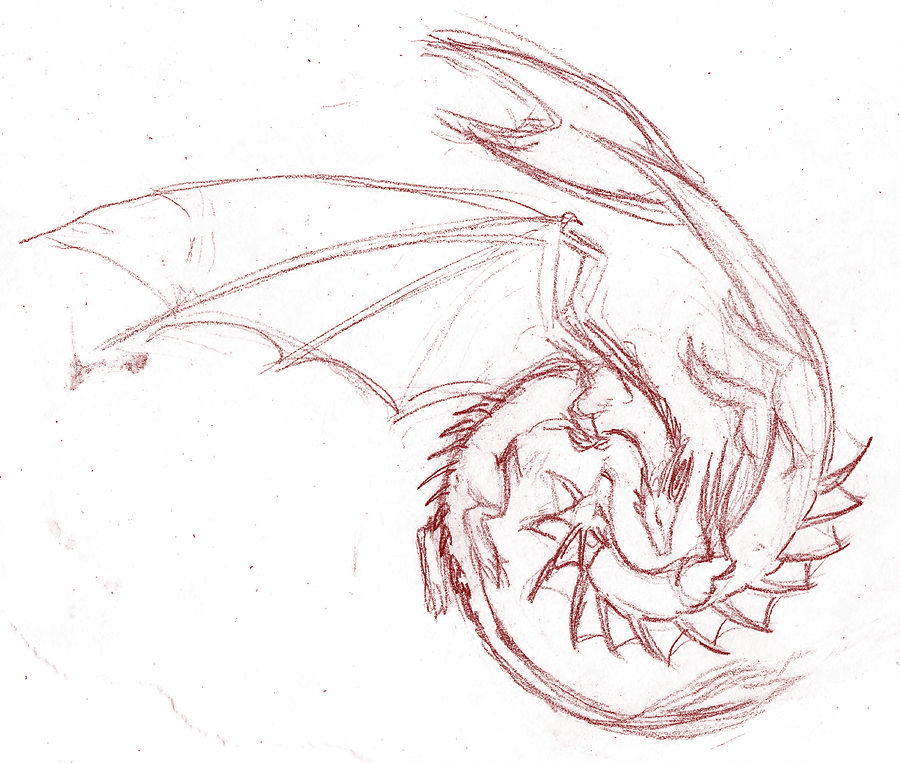
\includegraphics[width=\textwidth / 2 ]{img/drachen}
\end{figure}

%\chapter{Kapitel 2: Klassen}
\section{Elfen}
\textit{Hochnäsig aber freundlich.}

\subsection*{Namen}
Wenn ein Elf erwachsen wird sucht er sich einen neuen Namen aus. Davor wird er nach dem Kindernamen gerufen.\\
\textbf{Kindernamen:}\\
Ara, Bryn, Del, Eryn, Faen, Innil, Lael, Mella, Naill, Naeris, Phann, Rael, Rinn, Sai, Syllin, Thia, Vall\\
\textbf{Männliche Erwachsenennamen:}\\
Adran, Aelar, Armil, Arannis, Aust, Beiro, Berrian, Carric, Enialis, Erdan, Erevan, Calinndan, Hadarai, Heian, Himo, Immeral, Ivellios, Laucian, Mindartis, Paelias, Peren, Quariom, Riardon, Rolen, Soveliss, Thamior, Tharivol, Theren, Varis\\
\textbf{Weibliche Erwachsenennamen:}\\
Adrie, Althaea, Anastrianna, Andrastem Antinua, Bethrynna, Birel, Caelynn, Drusilia, Enna, Felosial, Ielenia, Jelenneth, Keyleth, Leshanna, Lia, Meriele, Mialee, Naivara, Quelenna, Quillathe, Sariel, Shanairra, Shava, Silaqui, Theirastra, Thia, Vadannia, Valenthe, Xanaphia

\subsection*{Alter}
Körperliche Reife, wie bei Menschen, schließt Lebenserfahrung mit ins Erwachsenwerden ein. Erwachsenenalter: 100 Jahre. Kann bis zu 750 Jahre alt werden.

\subsection*{Gesinnung}
Eine sanftere Ausprägung des Chaos. Schätzen und verteidigen Freiheit aller. rücksichtslos und heimtückisch

\subsection*{Größe}
Etwas kleiner als Menschen, weit unter 150cm und knapp über 180cm

\subsection*{Gewicht}
100-145 Pfund

\subsection*{Attributserhöhung}
$Geschicklichkeitswert + 2$

\subsection*{Bewegungsrate}
9 Meter / 30 Fuß / 3 Felder

\subsection*{Fähigkeiten}
\begin{itemize}
	\item Dunkelsicht
	\item Geschärfte Sinne
	\item Feenblut
	\item Trance
\end{itemize}

\subsection*{Sprachen}
\begin{itemize}
	\item Gemeinsprache, Elfisch
	\subitem lesen, schreiben, sprechen
\end{itemize}

\subsection*{Unterarten}
Zu Informationen und Werten zu den Unterarten siehe PH.
\begin{itemize}
	\item Hochelfen
	\item Waldelfen
	\item Dunkelelfen
\end{itemize}

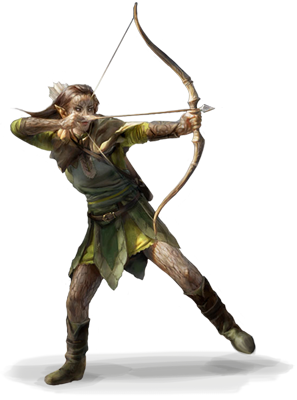
\includegraphics[width=\textwidth / 3]{img/elf} %70% der Textbreite

% ####################################################
%
% ####################################################

\newpage
\section{Halblinge}

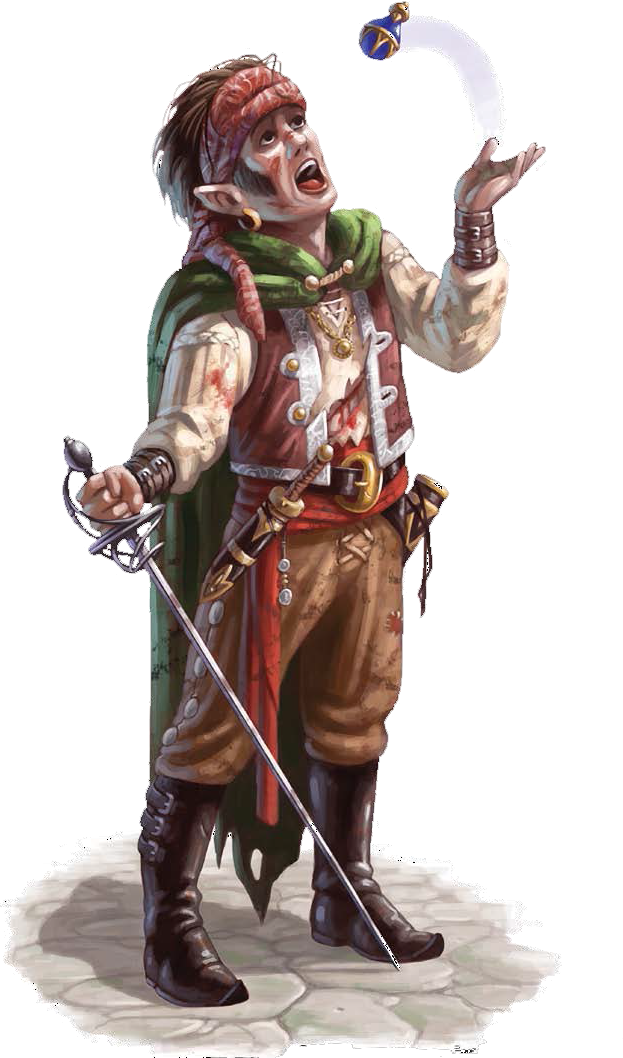
\includegraphics[width=\textwidth / 3]{img/halbling}

\textit{Umgänglich und positiv.}

\subsection*{Namen}
Jeder Halbling besitzt einen Vornamen, Familiennamen und möglicherweise einen Spitznamen. Bei Familiennamen handelt es sich oft um Spitznamen die so treffend waren, dass sie über Generationen hinweg weiter gegeben wurden\\
\textbf{Männliche Vornamen:}\\
Alton, Ander, Cade, Coorin, Eldon, Errich, Finan, Garret, Lindal, Lyle, Merric, Milo, Osborn, Perrin, Reed, Roscoe, Wellby\\
\textbf{Weibliche Vornamen:}\\
Andry, Bree, Callie, Cora, Euphemia, Jillian, Kithri, Lavinia, Merla, Nedda, Paela, Portia, Seraphina, Sheana, Trym, Vani, Verna\\
\textbf{Familiennamen:}\\
Buschsammler, Dickdorn, Fallkraut, Grünflasche, Goldbarren, Hochhügel, Hügelspitz, Strammgurt, Teeblatt, Unterast

\subsection*{Alter}
Ist mit 20 Jahre erwachsen. lebt ca. 150 Jahre.

\subsection*{Gesinnung}
Rechtschaffen gut. Mitfühlend, warmherzig und freundlich. Tollerieren keine Form der Unterdrückung.

\subsection*{Größe}
~ 90cm groß

\subsection*{Gewicht}
40 Pfund

\subsection*{Attributserhöhung}
$Geschicklichkeitswert + 2$

\subsection*{Bewegungsrate}
7,5 Meter / 22,5 Fuß / 2 Felder

\subsection*{Fähigkeiten}
\begin{itemize}
	\item Halblingsglück
	\item Tapferkeit
	\item Halblingsgewandheit
\end{itemize}

\subsection*{Sprachen}
\begin{itemize}
	\item Halblingisch, Gemeinsprache
	\subitem lesen, schreiben, sprechen
\end{itemize}

\subsection*{Unterarten}
Zu Informationen und Werten zu den Unterarten siehe PH.
\begin{itemize}
	\item Leichtfüße
	\item Stämmige
\end{itemize}

% ####################################################
%
% ####################################################

\newpage
\section{Menschen}

\textit{Jedermanns zweitbester Freund.}

\subsection*{Namen}
Keine spezifischen Namen. Für Inspiration können Namen aus den 9 Ethischen Gruppen verwendet werden. \textit{siehe Seite 28 im PH.}

\subsection*{Alter}
Ist mit 20 Jahre erwachsen. lebt wenigger als ein Jahrhundert.

\subsection*{Gesinnung}
Keine bestimmte Gesinnung.

\subsection*{Größe}
Kaum 150cm bis 180cm

\subsection*{Gewicht}
Schwankt stark

\subsection*{Attributserhöhung}
$Jeder Attributswert + 1$

\subsection*{Bewegungsrate}
9 Meter / 30 Fuß / 3 Felder

\subsection*{Fähigkeiten}
/

\subsection*{Sprachen}
\begin{itemize}
	\item Gemeinsprache, andere Sprache
	\subitem lesen, schreiben, sprechen
	\item Lernen häufig die Sprache mit denen sie am meisten zu tun haben.
	\item wollen belesen wirken und streuen Fremdworte in ihre Sprache.
\end{itemize}

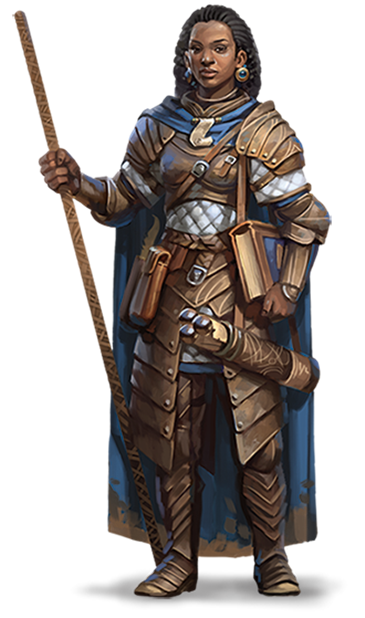
\includegraphics[width=\textwidth / 3]{img/human}


% ####################################################
%
% ####################################################

\newpage
\section{Zwerge}

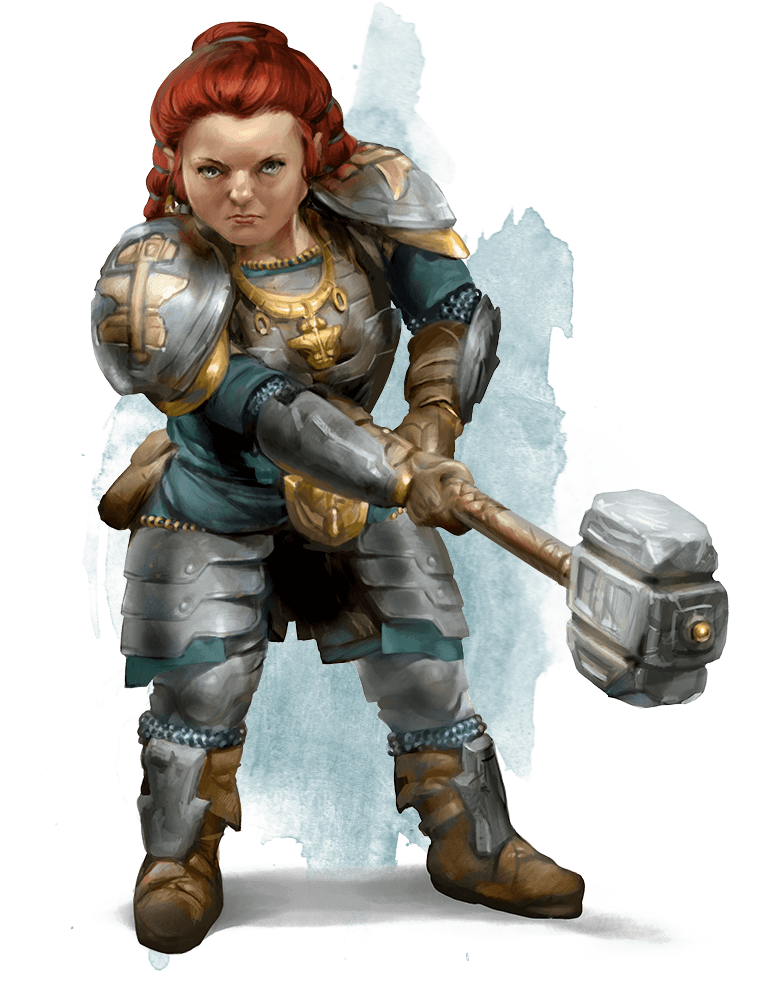
\includegraphics[width=\textwidth / 3]{img/zwerg}

\textit{Baut erst langsam Vertrauen auf und ist nachtragend wegen gutem Gedächtnis}

\subsection*{Namen}
Jeder Zwerg bekommt den Namen von dem Klanältesten verliehen. Bringt er Schande über diesen Namen wird es ihm per Gesetz verboten einen anderen Namen als diesen zu tragen.\\
\textbf{Männliche Vornamen:}\\
ADrik, Allberich, Baeren, Barendd, Bottor, Bruenor, Dain, Darrak, Delg, Eberk, Einkil, Fargrim, Flint, Gardain, Harbek, Kildrak, Morgran, Orsik, Oskar, Rangrim, Rurik, Taklinn, Thoradin, Thorin, Tordek, Traubon, Travok, Ulfgar, Veit, Vondal
\\
\textbf{Weibliche Vornamen:}\\
Amber, Artin, Audhild, Bardryn, Dagnal, Diesa, Eldeth, Falkrunn, Finellen, Gunndola, Gurdis, Helja, Hlin, Kathra, Kristryd, Ilde, Liftrasa, Mardred, Riswynn, Sannl, Torbera, Torgga, Vistra\\
\textbf{Klannamen:}\\
Balderk, Heldenhammer, Starkamboss, Dankil, Feuerschmiede, Frostbart, Gorunn, Holderheck, Eisenfaust, Loderr, Lutgehr, Rumnaheim, Strakeln, Torunn, Ungart

\subsection*{Alter}
Altern so schnell wie Menschen. Werden mit 50 noch als Jung angesehen. Werden ca. 350 Jahre alt.

\subsection*{Gesinnung}
Glauben an eine Durchstrukturierte Gesellschaft, also rechtschaffend. Glauben dass jeder es verdient hat an einer gerechten Ordnung teilzu haben.
\subsection*{Größe}
120cm-150cm

\subsection*{Gewicht}
150 Pfund

\subsection*{Attributserhöhung}
$Konstitutionswert + 2$

\subsection*{Bewegungsrate}
7,5 Meter / 22,5 Fuß / 2 Felder

Wird nicht durch das Tragen von schwerer Rüstung reduziert.

\subsection*{Fähigkeiten}
\begin{itemize}
	\item Dunkelsicht
	\item Zwergische Unverwüstbarkeit
	\item Zwergisches Kampftraining
	\item Handwerkliches Geschick
	\item Steingespür
\end{itemize}

\subsection*{Sprachen}
\begin{itemize}
	\item Zwergisch, Gemeinsprache
	\subitem lesen, schreiben, sprechen
\end{itemize}

\subsection*{Unterarten}
Zu Informationen und Werten zu den Unterarten siehe PH.
\begin{itemize}
	\item Gebirgszwerg
	\item Hügelzwerg
\end{itemize}

% ####################################################
%
% ####################################################

\newpage
\section{Drachenblütige}

\subsection*{Namen}
\subsection*{Alter}
\subsection*{Gesinnung}
\subsection*{Größe}
\subsection*{Gewicht}
\subsection*{Attributserhöhung}
\subsection*{Bewegungsrate}
\subsection*{Fähigkeiten}
\subsection*{Sprachen}
\subsection*{Unterarten}

% ####################################################
%
% ####################################################

\newpage
\section{Gnome}

\subsection*{Namen}
\subsection*{Alter}
\subsection*{Gesinnung}
\subsection*{Größe}
\subsection*{Gewicht}
\subsection*{Attributserhöhung}
\subsection*{Bewegungsrate}
\subsection*{Fähigkeiten}
\subsection*{Sprachen}
\subsection*{Unterarten}


% ####################################################
%
% ####################################################

\newpage
\section{Halbelfen}

\subsection*{Namen}
\subsection*{Alter}
\subsection*{Gesinnung}
\subsection*{Größe}
\subsection*{Gewicht}
\subsection*{Attributserhöhung}
\subsection*{Bewegungsrate}
\subsection*{Fähigkeiten}
\subsection*{Sprachen}
\subsection*{Unterarten}


% ####################################################
%
% ####################################################

\newpage
\section{Halborks}

\subsection*{Namen}
\subsection*{Alter}
\subsection*{Gesinnung}
\subsection*{Größe}
\subsection*{Gewicht}
\subsection*{Attributserhöhung}
\subsection*{Bewegungsrate}
\subsection*{Fähigkeiten}
\subsection*{Sprachen}
\subsection*{Unterarten}

% ####################################################
%
% ####################################################

\newpage
\section{Tiefling}

\subsection*{Namen}
\subsection*{Alter}
\subsection*{Gesinnung}
\subsection*{Größe}
\subsection*{Gewicht}
\subsection*{Attributserhöhung}
\subsection*{Bewegungsrate}
\subsection*{Fähigkeiten}
\subsection*{Sprachen}
\subsection*{Unterarten}

\chapter{Kapitel 2: Spielregeln}
\section{Würfel}
In DnD werden die Würfel 1 x W4, 1 x W6, 1 x W8, 2 x W10, 1 x W12 und 1 x W20 verwendet. Hierbei steht das W für Würfel (im Englischen meist D) und die Zahl für die Seitenzahl des Würfels.
\section{Spielablauf}
Eine Gruppe Abenteurern beschreiten ein Abenteuer, dass der Dungeon Master beschreibt. Der Ablauf einer Runde ist wie folgt: \\ \noindent \textbf{1) Der Spielleiter beschreibt die Umgebung} und erklärt die Grundlegenden Handlungsmöglichkeiten. \\
\noindent \textbf{2) Die Spieler beschreiben, was sie tun wollen}
\noindent Manchmal sind die Handlungen leicht und der DM wird die Konsequenzen der Handlung oder den Ort beschreiben, aber bei schwierigen Handlungen wird der Dungeon Master einen Würfelwurf verlangen und selbst den Ausgang der Handlung bestimmen. \\
\noindent \textbf{3) Der Spielleiter beschreibt die Auswirkungen der Spielerhandlungen.} Dies bringt die Spieler wieder zu Punkt 1).\\
\noindent  Im Kampf ist dieser Ablauf strukturierter, meisten jedoch passt sich der Ablauf flüssig an die Situationen an. Einige Dungeon Master verwenden auch Musik und/oder Miniaturfiguren.

\section{Attribute}
Spieler-Charaktere (PC) oder Nicht-Spieler-Charaktere (NPC) darunter auch Monster und zB Dorfbewohner haben alle \textbf{sechs verschiedene Attribute}:

\begin{itemize}
  \item Stärke
  \item Geschicklichkeit
  \item Konstitution
  \item Intelligenz
  \item Weisheit
  \item Charisma
\end{itemize}


\begin{minipage}{.45\linewidth}
	\begin{dndtable}
	   	\textbf{Punktzahl}  & \textbf{Modifikator} \\
			1 & -5 \\
			2-3 & -4 \\
			4-5 & -3 \\
			6-7 & -2 \\
			8-9 & -1 \\
			10-11 & +0 \\
			12-13 & +1 \\
			14-15 & +2 \\
	\end{dndtable}
\end{minipage}
\begin{minipage}{.45\linewidth}
	\begin{dndtable}
	   	\textbf{Punktzahl}  & \textbf{Modifikator} \\
			16-17 & +3 \\
			18-19 & +4 \\
			20-21 & +5 \\
			22-23 & +6 \\
			24-25 & +7 \\
			26-27 & +8 \\
		  28-29 & +9 \\
			30 & +0 \\
	\end{dndtable}
\end{minipage}

\section{Die Grundregeln}
\noindent Um das Resultat einer Handlung bestimmt werden soll, wird in DnD ein W20 verwendet. Dies gilt also für Attributs-, Angriffs-, und Rettungswürfe. \\
\noindent Der Ablauf:\\

\subsubsection*{}

\noindent \textbf{1) Würfeln}\\
Rechne den Modifikator drauf \\
\noindent \textbf{2) Bonus und Malus bedenken}\\
Ein Zauber, besondere Umstände- oder \\ andere Effekte\\
\noindent \textbf{3) Vergleichen}\\
Wenn der Wert den Minimalwert erreicht oder \\ übersteigt, dann ist der Wurf ein Erfolg.\\

\subsubsection*{}

\noindent Der vorgegebene Wert eines Attributs oder Rettungswurf ist der \textit{Schwierigkeitsgrad (SG)}. Für Angriffe ist es die \textit{Rüstungsklasse (RK)}. Dies wird alles später nochmal erwähnt.

\subsection{Vorteil und Nachteil}
Manchmal hast du einen Vorteil oder einen Nachteil auf einen Zauber oder eine Aktion. Dafür wirfst du zwei Würfel. Je nachdem ob Vorteil oder Nachteil verlangt wird, verwendest du den besten oder den schlechtesten Wurf der Beiden Würfe.
Falls du sowohl Nachteil als auch Vorteil auf eine Aktion hast, so verwendest du weder Vorteil noch Nachteil, auch wenn du zB zwei mal Vorteil und einmal Nachteil auf die Aktion hast. Mit dem Merkmal \textit{Halblingsglück} kann ein Held einen der Beiden noch einmal werfen.

\subsection{Attributswürfe}
Ein Attributswurf prüft das natürliche Talent und das Training eines Charakters oder Monsters, um eine Herausforderung zu bestehen.
Der DM kann Attributswürfe verlangen wenn eine Handung gelingen oder Misslingen kann (außer Anriffe).
Der Held würfelt dann mit einem W20 und wenn der Wurf nach dem einberechnen des Bonus / Malus größer / gleich dem SG ist, war der Wurf ein Erfolg.

\subsubsection{Übungsbonus}
Du kannst in einer Aufgabe, die mit einem Attributswurf zusammenhängt besonders gut sein. Du kannst nie mehr als eine Kompetenz einmal auf einen Wurf verrechnen.

\subsubsection{Vergleiche}
Wenn zwei Gestalten zB. ein Goblin (NPC) und ein Halbling (PC) gleichzeitig eine Aktion ausführen und sie nur einem von beiden gelingen kann, dass der Spielleiter eine Vergleichsprobe verlangt. Beide Charaktere werfen einen Wert und vergleichen ihn. Bei Unentschieden haben beide verloren. (Beispiel: Trinkspiele)

\subsubsection{Fertigkeiten}
Jedes Attrubut deckt eine breite Reihe von Fähigkeiten ab, darunter auch Fertigkeiten. in welcher ein Charakter geübt sein kann. Eine Fertigkeit repräsentiert einen bestimmten Aspekt eines Attributswertes: die Übung eines Charakters in einer Fertigkeit zeigt einen Scherpunkt auf diesen Aspekt.
Beispiel: Ein Charakter der die Fertigkeit Heimlichkeit besitzt hat Vorteile bei Würfen die mit Schleichen und Vertstecken zu tun haben. Die Folgenden Fertigkeiten gehören zu den jeweiligen Attributen.\\

\noindent \textbf{Stärkewurf}\\
\begin{itemize}
  \item Athletik
\end{itemize}
\noindent \textbf{Geschicklichkeitswurf}\\
\begin{itemize}
  \item Akrobatik
  \item Fingerfertigkeit
  \item Heimlichkeit
\end{itemize}
\noindent \textbf{Konstitutionswurf}\\
\begin{itemize}
  \item -
\end{itemize}
\noindent \textbf{Intelligenzwurf}\\
\begin{itemize}
  \item Arkane Kunde
  \item Geschichte
  \item Nachforschungen
  \item Naturkunde
  \item Religion
\end{itemize}
\noindent \textbf{Weisheitswurf}\\
\begin{itemize}
  \item Mit Tieren umgehen
  \item Motiv erkennen
  \item Heilkunde
  \item Wahrnehmung
  \item Überlebenskunst
\end{itemize}
\noindent \textbf{Charisma}\\
\begin{itemize}
  \item Täuschen
  \item Einschüchtern
  \item Auftreten
  \item Überzeugen
\end{itemize}

\subsection{Rettungswürfe}
EIn Rettungswurf stellt einen Versuch dar einem Zauber / einer Falle / einem Gift / einer Krankheit oä. zu widerstehen. Dazu würfelst du mit einem W20. Ein Rettungswurf kann auch durch Situationsbedingte Boni und Mali modifiziert werden.

\chapter{Kapitel 3: Kampfregeln}
\section{Kampfreihenfolge}
Kämpfe sind meist unübersichtlich, deshalb Ordnet das Spiel den Kampf in Runden und Züge ein.
Eine \textbf{Runde} sind in der Spielwelt ungefähr \textit{6 Sekunden}. Jeder Charakter macht während jeder Runde einen \textbf{Zug}.\\
Am Anfang wird die Reihenfolge der Charaktere Festgelegt indem jeder auf Initiative wirft .

\begingroup
\setthemecolor[PhbTan]

\begin{paperbox}{Kampf - Kurz und Knapp}
  \begin{enumerate}
    \item \textbf{Überraschungsmoment.} Der DM legt fest ob irgend ein Kampfbeteiligter überrascht wird.
    \item \textbf{Positionen bestimmen.} Der Spielleiter legt fest wo sich alle Spieler befinden beruhend auf den letzten Aussagen der Spieler. In welcher Entfernung und in welcher Richtung.
    \item \textbf{Initiative auswürfeln.} Alle Spieler erwürfeln mit einem Initiativewurf ihre Zugreihenfolge.
    \item \textbf{Züge.} Jeder Kampfbeteiligter macht einen Zug.
    \item \textbf{Neue Runde.} Nachdem jeder einen Zug gemacht hat fängt die nächste Runde an. Wiederholt ab Schritt 4 bis der Kampf vorbei ist.
  \end{enumerate}
\end{paperbox}
\endgroup

\subsection{Überraschung}
Wenn eine Seite vor dem Kampf einen \textit{Geschicklichkeitswurf (Heimlichkeit)} macht, vergleicht der DM jeden dieser Würfe mit dem Wert \textit{passive Warhnehmung} der zu Überraschenden Charaktere. Jeder der eine Bedrohung nicht bemerkt wird überrascht. Wenn ein Spieler Überrascht wurde, kann er sich bei seinem ersten Zug weder bewegen noch eine Aktion ausführen.

\subsection{Initiative}
Für Spieler ist es Selbsterklärend.
Für Monster: Der Spielleiter Würfelt einmal für eine ganze Gruppe identischer Kreaturen, sodass jede Kreatur einer Gruppe gleichzeitig handelt.
Bei Gleichstand unter Spieler entscheiden die Spieler.
Bei Gleichstand bei Kreaturen und Spieler entscheidet der DM. Ein höherer Wert kommt früher an die Reihe.

\subsection{Dein Zug}
Dein Zug besteht aus \textbf{bewegen} und das Ausführen einer \textbf{Aktion}. Du entscheidest ob du dich erst bewegen oder erst die Aktion ausführen möchtest. Du darfst auch darauf verzichten was zu tun. Wenn du nicht weißt was du tun sollst, empfielt sich eine \textit{Ausweich-} oder \textit{Bereitmach-} Aktion. Auf die genauen Aktionen werden wir später noch eingehen.

\subsubsection{Bonusaktionen}
Klassenmerkmale, Zabuer oder andere Fähigkeiten erlauben es dir eine Bonusaktion durchzuführen. Du kannst in deinem Zug nur eine Bonusaktion durchführen.

\subsubsection{Andere Aktivitäten in deinem Zug}
Dein Zug kann noch weitere Handlungen beihalten. Du darfst
\begin{itemize}
  \item So gut du es gerade kannst kommunitieren
  \item Mit Objekten in deiner Nähe interagieren. zB Türen öffnen oder Waffen ziehen. (Wenn du mit einem zweiten Gegenstand interagieren willst, musst du dies als Aktion tub)
\end{itemize}
Manche magische Gegenstände erfordern immer eine Aktion. Der DM kann von dir verlangen jede dieser Aktivitäten eine Aktion zu benutzen, solange sie besonderen Aufwand erfordert oder eine Art hinderniss ist.

\subsection{Reaktion}
Bestimmte besondere Fähigkeiten, Zauber und Situationen erlauben es dir eine Reaktion auszuführen. Du kannst nur eine Reaktion pro Runde ausführen.

\section{Bewegung und Positionen}
Bei einer Bewegung kannst du höchstens eine Distanz laufen, die deiner Bewegungsrate entspricht. Wieviel du davon verwendest ist dir überlassen. Deine Bewegung kann auch springen, klettern oder schwimmen beinhalten. Mehr dazu in Kapitel 3.
\subsection{Bewegung aufteilen}
Du kannst deine Bewegung in deinem Zug aufteilen, also zB deinen Zug so gestalten:
\begin{enumerate}
  \item Bewegung
  \item Aktion
  \item Rest der Bewegung
\end{enumerate}

\subsection{Schwieriges Gelände}
Schwieriges Geländer sind unteranderem Trümmer, Unterholz, steile Treppen, hoher Schnee und seichter Morast. Aber auch Bereiche in dem andere Figuren stehen. Will eine Figur sich in schwierigem Gelände fortbewegen kostet sie jeder Meter einen weiteren.

\subsection{Am Boden Liegend}
Wenn du niedergeschlagen wurdest oder dich zB selbst auf den Boden geworfen hast. Aufstehen kostet dich die hälfte deiner Bewegungsrate. Um dich zu bewegen während du am Boden liegst musst du \textit{kriechen} oder Magie benutzen. Wenn du kriechst kostet jeder Meter einen weiteren. Auf schwierigem Gelände also insgesamt 3 Meter für 1 Meter Bewegung.

\subsection{Sich um andere herum Bewegen}
Du kannst dich durch ein Bereich einer nichtfeindlichen Figur bewegen. Möchtest du dich durch ein Bereich bewegen auf dem eine andere nichtfeindliche Figur steht, muss sie mindestens zwei Größen größere oder kleiner ist als du sein.
Wenn du dich aus der Reichweite eines Feindes bewegst provozierst du einen Gelegenheitsangriff.

\section{Aktionen im Kampf}
Der DM entscheidet ob diese Aktion möglich ist. Wenn ja wird er dir sagen welchen Wurf du ablegen musst.

\subsection{Angriff}
Du führst einen Fern- oder Nahkampf aus. Näheres dazu in \textit{Angreifen}. Durch Merkmale kannst du auch zweimal Angreifen. (zB. Kämpfer ab lv. 5: \textit{Zusätzlicher Angriff})

\begingroup
\setthemecolor[PhbTan]
\begin{paperbox}{Zaubersprüche}
  Zauberwirkende wie zB Magier oder Kleriker (oder andere magische Wesen) können auf Zauber verwenden. Jeder Zauber hat einen Zeitaufwand, der Festlegt ob der Zauberwirkendeeine Aktion, Reaktion, Minuten oder sogar Stunden aufwenden muss, um den Zauber wirken zu lassen. Die meisten Zauber haben aber einen Zeitaufwand von einer Aktion. Siehe Kapitel 4 für die Zauberregeln.
\end{paperbox}
\endgroup

\subsection{Ausweichen}
Wenn die Bewegungsrate > 0 und du nicht kampfunfähig bist:
Jeder Angriff bis zu deinem nächsten Zug erhält einen Nachteil, wenn du den Angreifer sehen kannst. Du bekommst einen Vorteil auf Rettungswürfe (Geschicklichkeit).

\subsection{Gegenstand verwenden}
Normalerweise Interagierst du mit einem Gegenstand während du zB als Teil deines Angriffes dein Schwert ziehst. Wenn ein Gegenstand aber eine Aktion verlankt oder es die zweite Interaktion mit einem Gegenstand ist brauchst du diese Aktion um ihn zu verwenden.

\subsection{Helfen}
Die Kreatur der du hilfst bekommt einen Vorteil auf den nächsten Attributswurf, wenn sie den Wurf vor Beginn des nächsten Zuges macht. Bei einem Angriff darfst du nur einer Figur helfen die 1,5m von dir entfernt ist.

\subsection{Rückzug}
Du provozierst \textbf{keinen} Gelegenheitsangriff.

\subsection{Spurt}
Deine Bewegungsrate verdoppelt sich.

\subsection{Suchen}
Du lenkst die Aufmerksamkeit darauf was zu finden. Der DM kann einen Weisheitswurf(Wahrnehmung) oder Intelligenzwurf(Nachforschung) verlangen.

\subsection{Verstecken}
Du kannst dich verstecken, der DM kann einen Geschicklichkeitswurf(Heimlichkeit) verlangen. Wenn er gelingt erhälst Vorteile (siehe Unsichtbare Angreifer und Ziele).

\subsection{Bereit machen}
Diese Aktion verwendest du, wenn du einem Feind zuvorkommen willst. Du kannst dadurch später in der Runde eine Reaktion ausführen.
\begin{enumerate}
  \item Wähle einen wahrnehmbaren Zustand der die Reaktion auslöst
  \item Wähle die Aktion die als Antwort eingesetzt wird
\end{enumerate}
Beispiel: "Wenn der Goblin in die Luft springt, lege ich den Hebel für die Falltür um."
Wenn ein Zauber auf diese Art vorbereitet wird, kannst du ihn ganz normal einsetzen und seine Energie noch zurückhalten, die du dann in der Reaktion entfesselst. (Du benötigst bis zum Zeitpunkt des einsetzen des Zaubers Konzentration. Siehe Kapitel 4)


\section{Angreifen}
Ablauf eines Angriffes:
\begin{enumerate}
  \item Wähle ein Ziel dass in deiner Reichweite bist
  \item Lege die Modifikatoren fest
  \item Führe den Angriff aus
  \item Bei einem Treffer: Schaden auswürfeln, es sei denn was anderes wird verlangt
\end{enumerate}

\subsection{Angriffswürfe}
Der Angriffswurf legt fest ob du triffst. Würfel mit einem W20 und addiere die Modifikatoren. Wenn dieser Wert größer gleich der Rüstungsklasse des Ziels ist trifft der Angriff

\subsubsection{Modifikatoren auf den Wurf}
Die zwei häufigsten Modifikatoren sind Übungsboni und Attributsmodifikatoren. Wenn du mit der Waffe mit der du angreifst darfst du den Übungsbonus zu dem Wert Addieren, der Attributsmodifikator steht auf deinem Charaktersheet. Die Werte der Monter stehen im Abenteuerbuch.

\subsubsection{1er \& 20er}
Wenn du mit einem W20 eine 20 würfelst dann trifft der Angriff ohne Rücksicht auf Modifikatoren oder die RK des Gegners. Zudem ist der Angriff ein kritischer Treffer. Bei einer 1 verfehlt der Angriff direkt.

\subsection{Ungesehene Angreifer und Ziele}
Wenn du ein Ziel angreifst, dass du nicht sehen kannst hast du einen Nachteil auf deinen Wurf. Auch wenn du die Position erraten musst oder du dein Ziel nur hörst. Der DM sagt dir nur ob dein Angriff missglückt ist nicht ob du die Stelle erraten hast.

\subsection{Fernkampfangriffe}
Nicht nur Fernkampfwaffen, auch viele Zauber enthalten einen Fernkampfwurf.

\subsubsection{Reichweite}
Du kannst nur Ziele innerhalb deiner Reichweite wählen. Manche Fernkampfwaffen haben 2 Reichweiten. Die kleienre Zahl ist die minimal die größere die Maximal Reichweite. Dein Wurf erleidet einen Nachteil, wenn die Zahl nicht größer / gleich des Minimalwertes der Reichweite ist und nicht den Maximalwert überschreitet.

\subsubsection{Fernkampf im Nahkampf}
Wenn ein Gegner im Umkreis von 1,5m bei dir steht erhälst du auf deinen Angriffswurf einen Nachteil.

\subsection{Nahkampf Angriffe}
Du kannst nur Kreaturen in deiner Umgebung angreifen. Die meisten haben 1,5m als Reichweite. Du kannst auch einen \textbf{Waffenlosen Schlag} ausführen. Ein Fausthieb, Tritt, etc. Addiere Übungsbonus und den Stärkemod. zu deinem Angriffswurf. Wenn du triffst, teilst du 1 + Stärkemodifikator Wuchtschaden aus. DU bist immer geübt in Waffenlosen Schlägen.

\subsection{Gelegenheitsangriff}
Wenn du versuchst achtlos an einem Feind vorbei zu spazieren provozierst du einen Gelegenheitsangriff. Du kannst Gelegenheitsangriffe Ausführen wenn eine Kreatur, die sichtbar für dich ist aus deiner Reichweite hinaus bewegt. Du verwendest eine Reaktion für einen Nahkampfangriff, die die Bewegung der Kreatur unterbricht bevor sie aus deiner Reichweite austritt. Durch eine Rückzugsaktion oder durch Teleportation vermeidest du ihn.

\subsection{Zwei-Waffen-Kampf}
Wenn du mit einer leichten Nahkampfwaffe einen Angriff ausführst erhälst du eine zusätzliche Aktion, die du verwenden kannst um mit einer weiteren Nahkampfwaffe anzugreifen. Bei der Besonderheit "Wurfwaffe" kannst du die Waffe auch werfen. Du addierst aber keinen Attributsmodifikator zu dieser Waffe, es sei denn er ist negativ.

\section{Deckung}
\noindent Wenn Objekte dir Deckung bieten wird es schwieriger das Ziel zu verletzen. \\
\noindent \textbf{Halbe Deckung:} +2 RK und +2 Rettungswurf\\
\noindent \textit{(niedrige Mauer / Möbelstück / schmaler Baumstamm / Kreatur (egal ob Freund oder Feind)}\\
\noindent \textbf{Dreiviertel Deckung:} +5 RK und +5 Rettungswurf \\
\noindent \textit{(Fallgitter / Schießscharte / dicker Baumstamm)}\\
\noindent \textbf{Vollständige Deckung:} kann nicht direkt angegriffen werden außer durch einige Zauber.\\

\section{Schaden und Heilung}
\subsection{Trefferpunkte}
Repräsentiert eine Kombination vo körperlicher und geistiger Widerstandsfähigkeit. Der Verlust der Trefferpunkte hat keinen Effekt auf die Fähigkeiten der Kreatur bis die Zahl auf 0 fällt.

\subsection{Schadenswürfe}
Man würfelt Schaden mit dem/den Schadenswürfel/n, addiert die Modifikatoren und wendet sie auf das Ziel an. Magische Waffen. besondere Fähigkeiten oder andere Faktoren können einen Bonus auf den Schaden erlauben (nicht der Übungsbonus).
Rechne den Attributsmodifikator den du in deinem Angriffswurf verwendet hast zu dem Schaden hinzu. Ein Zauber sagt dir mit welchen Würfeln und welche Modifikatoren du verwenden musst. Bei mehreren Zielen würfelst du für alle Ziele den Schaden gleichzeitig aus.

\subsubsection{Kritische Treffer}
Bei einem kritischen Treffer würfelst du zweimal mit den Schadenswürfel und addierst sie. Zähle danach Modifikatoren hinzu.

\subsubsection{Schadensarten}
Schadensarten haben keine eigenen Regeln aber andere Regeln wie Schadensresistenz basieren auf ihnen.
\textit{Blitzschaden, Energieschaden, Feuerschaden, Giftschaden, gleißender Schaden, Hiebschaden, Kälteschaden, nekrotischer Schaden, psychischer Schaden, Säureschaden, Schallschaden, Stichschaden, Wuchtschaden}

\subsection{Schadensresistenz und Anfälligkeit}
Manche KReaturen und Gegenstände sind \textbf{resistenter} \textit{(Schaden wird halbiert)} und/oder \textbf{anfälliger} \textit{(Schaden wird verdoppelt)} für bestimmte Schadensarten.
Anfälligkeit und Resistenz werden nach allen anderen Schadensmodifikatoren angewendet. Besitzt eine Kreature mehrere, dann gelten sie als nur eine bei einem Angriff.

\subsection{Heilung}
Schaden ist nicht permanent und sogar der Tod ist durch mächtige Magie umkehrbar. \textit{Rast} oder \textit{Magie} können die Trefferpunkte einer Kreatur wiederherstellen. Die Punkte können bei Heilung nicht den Maximalwert übersteigen.

\subsection{0 Trefferpunkte}
Wenn du auf 0 Trefferpunkte fällst, stirbst du entweder sofort oder verlierst das Bewusstsein, wie in den folgenden Abschnitten erklärt wird. Die meisten SL lassen Monster sterben, sobald ihre Trefferpunkte auf 0 fallen, anstatt sie das Bewusstsein verlieren und einen Rettungswurf ablegen zu lassen. Mächtige Bösewichte und besondere NSC sind oft Ausnahmen; der SL kann sie in Ohnmacht fallen und den gleichen Regel folgen lassen, die für die Spieler gelten.

\subsubsection{Sofortiger Tod}
Wenn der Schaden deine TP auf 0 reduzieren und noch Schaden übrig ist stirbst du sofort, wenn der übrige Schaden größer/gleich deinem Trefferpunkte maximum ist.

\subsubsection{Bewusstsein verlieren}
Wenn du nicht tod bist wirst du Bewusstlos. Die Bewusstlosigkeit endet wenn du TP zurückgewinnst.

\subsubsection{Todesrettungswürfe}
Wenn du einen Zug mit 0 TP beginnst musst du einen Todesrettungswurf ablgen. Dieser Rettungswurf ist an kein Attribut gebunden, du kannst aber Zauber und besondere Fähigkeiten als Unterstützung verwenden Würfele mit einem W20 bei 10 oder höher ist er gelungen. Bei deinem dritten Erfolg bist du stabilisiert. Bei deinem dritten Fehlschlag stirbst du. Sie müssen nicht nacheinander erfolgen.\\
\noindent \textbf{1er und 20er:}\\
\ \ 1: Dieser Fehlschlag zählt doppelt.\\
\ \ 20: Du erhälst einen TP zurück.\\
\noindent \textbf{Schaden bei 0 Trefferpunkten:}\\
\ \ Zählt als Fehlschlag beim Rettungswurf gegen den Tod. Bei kritischem Treffer zählt er als zwei. Wenn der Schaden deinem TP maximum übersteigt stirbst du sofort.

\subsubsection{Stabilisieren}
Wenn heilung nicht möglich ist kann eine Kreatur stabilisiert werden. Du kannst eine Aktion verwenden um bei einer Kreatur Erste-Hilfe zu leisten. Erfoderlich dafür ist ein \textit{Weisheitswurf(Heilkunde)} mit SG 10. Ist eine Kreatur stabil wirft sie keine Rettungswürfe gegen den Tod mehr ab, erhält nach 1W4 Stunden einen TP, bleibt aber Bewusstlos. Sobald sie Schaden erleidet ist sie nicht mehr stabil.

\subsection{Bewusstlos schlagen}
Schlägt eine Kreatur eine andere mit einem Nahkampfangriff auf 0 TP, so kann die Figur während dem Schlag entscheiden, ob der Schlag den Gegner nur ausnocken soll. Ist eine Figur Bewusstlos, so ist sie stabil.

% \chapter{Bildquellen}

\begin{itemize}
  \item drachen
  \subitem https://www.deviantart.com/chardove/art/Dragon-Doodle-321625831

  \item Elfe
  \subitem http://pngimg.com/download/47334

  \item Halbling
  \subitem https://de.kisspng.com/png-z2wr4a/preview.html

  \item Mensch, Zwerg
  \subitem DnD Beyond

\end{itemize}

\end{document}
